\documentclass{article}
\usepackage[utf8]{inputenc}

\title{Beautiful Empathy}
\date{December 2020}

% \usepackage{natbib}
\usepackage{graphicx}
\usepackage{amsmath}
\newcommand{\lvl}[1]{\vspace{0.5cm}\Large{\textbf{#1}}\vspace{0.2cm}}

\begin{document}

\maketitle

\textit{Author}: dariogarcia@gmail.com

\begin{figure}[h!]
\centering
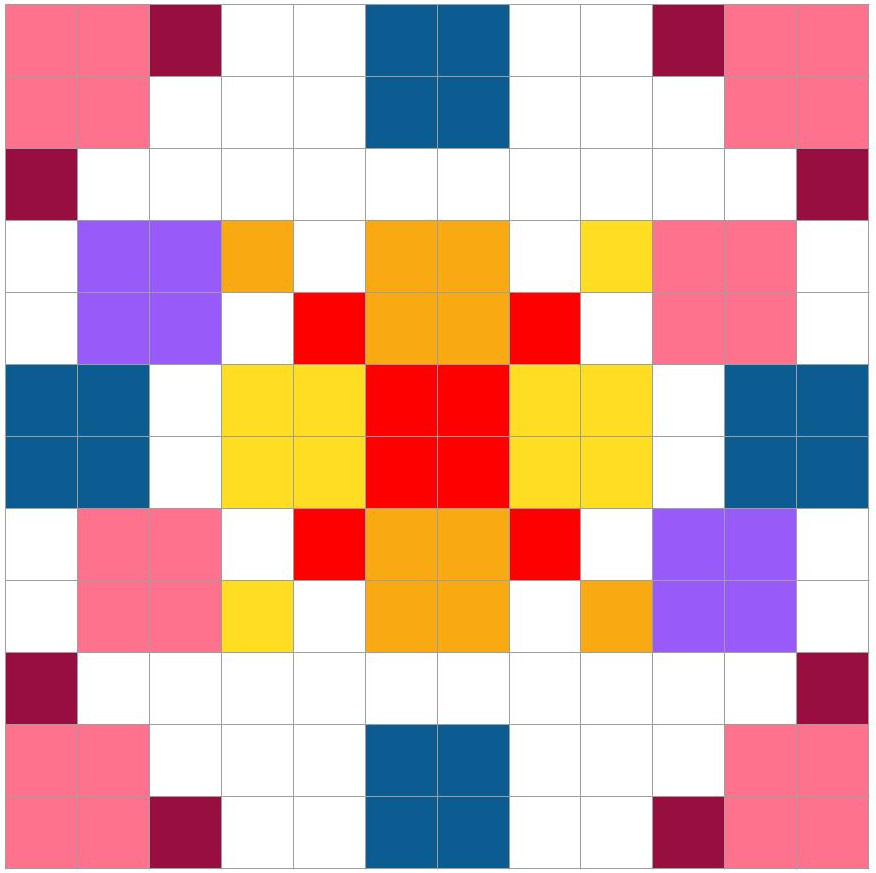
\includegraphics[scale=0.2]{First_ever.jpg}
\caption{First ever mosaic created in Beautiful Empathy}
\label{fig:mosaic}
\end{figure}


\lvl{Beautiful Empathy}

Beautiful Empathy is a collaborative board game, the goal of which is to create a colored mosaic. The game has no scoring system and there is no official winner. Beautiful Empathy is conceived as a two player game, but the rules can be easily adapted to host more players. 


\lvl{Game Script}

Beautiful Empathy is played in a series of turns. On each turn, one player is the guesser and the other the painter. At the beginning of each turn freely decide who is who. Once decided, the turn starts with the guesser, who tries to figure out which word would the painter use to complete a sentence (out of two optional words). For example:

\begin{centering}
\texttt{Sentence:}\\
\textit{The tree was --------- in the middle of the forest}
\texttt{Options:}\\
\textit{shaking} | \textit{shinning}\\
\end{centering}
\vspace{0.5cm}

After the round of 5 questions, count the number of correct ones.
More correct answers by the guesser will give more options for the painter on the second part of the turn. 

During this part, the painter may first gain a color to its palette. Afterwards, it can draw cards to see the shapes which will be placed on the mosaic. The painter can use any combination of colors in its palette when placing the tiles. Once all tiles have been placed, the turn is over and a new one can begin.


\lvl{Getting Colors}

Each player starts the game with one random color.

After the correct questions have been counted, the painter may gain a new color. This happens if the number of correct answers is bigger than the number of already owned colors. For example, a painter who owns 2 colors will get a new color if 3 or more questions were correctly answered by the guesser. Five correct answers will always get the painter a new color, regardless of the colors already owned.

The painter can choose the color to gain, among those directly connected in the color map with a color he or she already owns. Mark the colors each player owns in the color map.

\begin{figure}[h!]
\centering
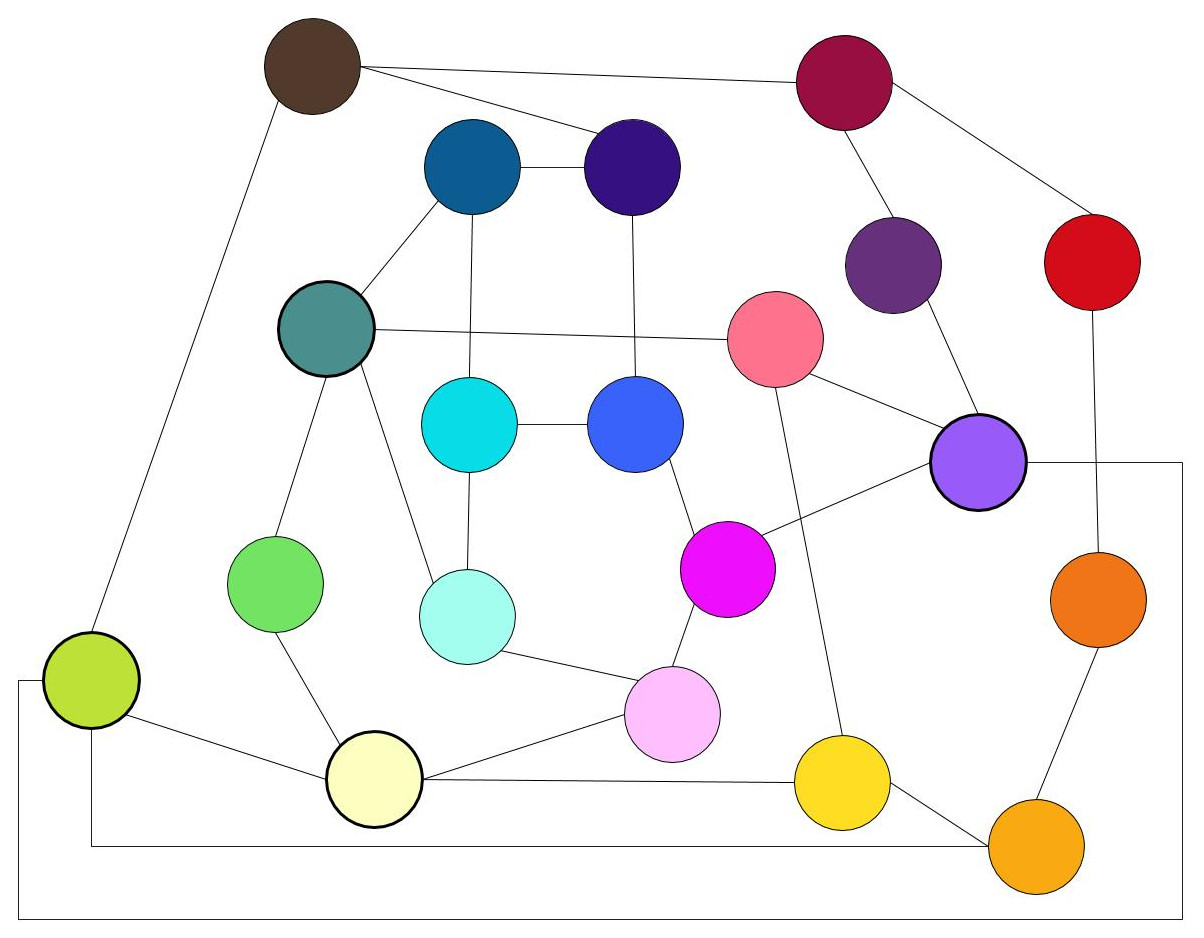
\includegraphics[scale=0.25]{color_map.jpg}
\caption{Color map. Edges between colors indicates direct connection.}
\label{fig:color_map}
\end{figure}


\lvl{Picking Shapes}

After the getting colors phase, the painter must choose the shapes to place on the mosaic. To do so, the painter must draw a card from one of two decks. Additionally, if the guesser got 5 correct answers, a bonus action for the painter is gained. In details:

\begin{itemize}
    \item If 1 or less questions were correctly guessed, draw from deck 1. This includes the following distribution:
    \begin{itemize}
        \item 70\%: 4 small squares
        \item 20\%: 4 small squares + 1 big square (2x2)
        \item 10\%: 8 small squares
    \end{itemize}
    \item If 2 or more questions were correctly guessed, draw from deck 1. This includes the following distribution:
    \begin{itemize}
        \item 20\%: 8 small squares
        \item 40\%: 4 small squares + 2 big squares (2x2)
        \item 30\%: 8 small squares + 2 big squares (2x2)
        \item 10\%: 16 small squares
    \end{itemize}
\end{itemize}

If the 5 answers were correct, additionally to the previous selection, one bonus card is drawn. The bonus deck contains the following options with uniform distribution:
\begin{itemize}
    \item Gift any one color to your companion.
    \item Occupy 8 tiles with any colors of your choice.
    \item Change the color of 4 tiles already in the board.
\end{itemize}


\lvl{End of Game}

The Game ends when the players agree to, or when a player cannot place its tiles because of lack of space on the mosaic. Once this is done, take a look at the mosaic you created through empathy, and enjoy it!

% \bibliographystyle{plain}
% \bibliography{references}
\end{document}
